\chapter{Uczenie maszynowe}
\label{cha:ucz.masz}

Uczenie maszynowe (ML, od ang. \textit{machine learning}) to nauka o~algorytmach komputerowych, które automatycznie ulepszają się dzięki doświadczeniu i~wykorzystaniu danych \cite{Mitchell97}. Algorytmy uczenia maszynowego są budowane na podstawie przykładowych danych, zwanych „danymi szkoleniowymi”, w~celu prognozowania lub podejmowania decyzji bez bezpośredniego zaprogramowania do tego \cite{Koza96}. Natomiast nieco bardziej techniczną definicję uczenia maszynowego przedstawił Tom Mitchell w~1997 roku: \textit{Mówimy, że program komputerowy uczy się na podstawie doświadczenia $E$ w~odniesieniu do jakiegoś zadania $T$ i~pewnej miary wydajności $P$, jeśli jego wydajność (mierzona przez $P$) wobec zadania $T$ wzrasta wraz z~nabywaniem doświadczenia $E$}.

Dyscyplina uczenia maszynowego wykorzystuje różne podejścia do uczenia modeli wykonywania zadań, w~przypadku których nie jest dostępny w~pełni zadowalający algorytm. Wstęp do uczenia maszynowego wraz z~wyjaśnieniem pojęć podstawowych został przedstawiony w~rozdziale \ref{cha:pojecia}. Główne nurty zostały zaprezentowane w~rozdziale \ref{cha:cha3.2}. Natomiast w~kolejnych podrozdziałach zostały zaprezentowane metody dotyczące przygotowannia danych. Ostatnie podrozdziały dotyczą metod  uczenia maszynowego, które zostały wykorzystane w~trakcie badań.

\section{Pojęcia podstawowe}
\label{cha:pojecia}

Jednym z~podstawowych terminów w~uczeniu maszynowym jest \textbf{atrybut} (ang. \textit{attribute}). Oznacza on konkretny typ danych (np. wiek). Innym terminem jest \textbf{cecha} (ang. \textit{feature}), która oznacza atrybut wraz z~jego wartością. Mają one zastosowanie między innymi w~przypadku danych w~postaci plików csv. Aby móc skorzystać z~mocy uczenia maszynowego, musimy wybrać jakiś model, który wytrenujemy. Modele zostały opisane w~rozdziale \ref{cha:Wykorzystane metody uczenia maszynowego}, natomiast ogólne typy uczenia maszynowego w~rozdziale \ref{cha:cha3.2}. Jednakże, zanim ostatecznie zdecydujemy się który model powinien być wykorzystany, należy porównać istniejące modele. W~tym celu zazwyczaj wykorzystuje się \textbf{funkcję kosztu}, która mówi nam jak duży błąd popełnia model podczas predykcji \cite{Sawka18}. 

Innym aspektem związanym z~modelami uczenia maszynowego jest to, jakie wyniki osiąga dany model (również względem posiadanych danych). Jednym z~problemów z~tym związanych jest tzw. \textbf{przetrenowanie}, bądź też inaczej, \textbf{nadmierne dopasowanie} (ang. \textit{overfitting}). Oznacza to, iż model bardzo dobrze sobie radzi na danych uczących, natomiast dla danych testowych wyniki są już o~wiele gorsze. Jest to równoznaczne z~tym, iż model nie uogólnia danych zbyt dobrze. Zdarza się to najczęściej, gdy mamy zbyt małą ilość danych i~dodatkowo użyjemy zbyt skomplikowanego modelu. Jest to dosyć znany problem, który występuje w~literaturze pod nazwą kompromis między obciążeniem a~wariancją (ang. \textit{bias-variance tradeoff}). Istnieje wiele rozwiązań, które zapobiegają przetrenowaniu. Jednym z~nich jest \textbf{regularyzacja}. To, jak bardzo chcemy regularyzować proces uczenia zależy od tego, jakie wartości przypiszemy \textbf{hiperparametrom} (ang. \textit{hyperparameters}). 

Analogicznym problemem jest \textbf{niedotrenowanie} (ang. \textit{underfitting}), jednakże w~tym przypadku chodzi o~dokładnie przeciwne zjawisko, tzn. gdy model jest zbyt prosty (w stosunku do danych). W~tym przypadku istnieje kilka rozwiązań, jak \cite{Sawka18}:
\begin{itemize}
\item
wybór mocniejszego modelu (który posiada większą liczbę parametrów),
\item
zmodyfikowanie danych w~taki sposób, aby posiadały większą liczbę cech (patrz rozdział \ref{cha:cha3.3}),
\item
redukcja regularyzacji (bądź innych ograniczeń modelu).
\end{itemize} 
  
Kolejnym problemem związanym ze słabymi wynikami modelu jest aspekt dotyczący danych. Pierwsze utrudnienie to zbyt mała liczba danych. W~zależności od zagadnienia wymagana liczba przykładów uczących może się wahać między setkami (np. predykcja obecności choroby u pacjenta na podstawie danych zdrowotnych) a~milionami (np. rozpoznawanie mowy, klasyfikacja tekstu). Kolejnym problemem związanym z~danymi jest zaszumienie danych. Innymi słowy, mamy z~taką sytuacją do czynienia, gdy dane nie odzwierciedlają rzeczywistości (a przynajmniej nie całkowicie poprawnie). Wtedy, niezależnie od zastosowanego modelu nie ma możliwości, aby system, mając do dyspozycji niereprezentatywne dane, radził sobie dobrze na danych testowych. Dotyczy to również przypadków, gdy dane są błędne. Rozwiązaniem tego problemu może być przykładowo \cite{Sawka18}:
\begin{itemize}
\item
odrzucenie elementów odstających,
\item
odrzucenie, bądź uzupełnienie brakujących danych,
\item
rozpoznanie i~odrzucenie błędnych danych.
\end{itemize}

Ostatnim poruszonym zagadnieniem  związanym z~danymi są nieistotne cechy. Mogą one działać jak szum i~obniżać jakość posiadanych danych. W~tym przypadku rozwiązaniem może być odrzucenie nadmiarowych cech i~uproszczenie danych. Kwestia ta zazwyczaj jest poruszana w~trakcie wykonywania inżynierii cech (patrz rozdział \ref{cha:cha3.3}).
Gdy już posiadamy wyuczony model, dobrze byłoby upewnić się, iż działa on tak, jak powinien. Podejście, które się utrwaliło jest podział posiadanych danych na zbiory \textbf{danych uczących} oraz \textbf{danych testowych} (czasami również odkłada się jeszcze jeden zbiór danych walidacyjnych, aby we wczesnej fazie wyszukiwania odpowiedniego modelu sprawdzać wyniki właśnie na tych danych, a~po wybraniu ostatecznego modelu, przetestować jego skuteczność na danych testowych). Zazwyczaj 80\% wszystkich danych przeznacza się na dane uczące \cite{Sawka18}.

Docelowym zadaniem, które będzie badane w~tej pracy jest klasyfikacja wytrzymałości odlewów na podstawie mikrostruktur. Dane, jakimi dysponujemy posiadają dwie etykiety: niska oraz wysoka wytrzymałość (bądź też inny wskaźnik). A~więc trzeba będzie skorzystać z~\textbf{klasyfikatora binarnego}. Jak natomiast zweryfikować jak dobrze sobie radzi dany klasyfikator? Aby to stwierdzić w~statystyce używa się wielu miar, które pokrótce zostaną tutaj przedstawione. Zacznijmy od wyjaśnienia takiego pojęcia jak \textbf{tablica pomyłek}. W~klasyfikacji binarnej dane są oznaczone dwiema etykietami, dla uproszczenia nazwijmy je \textbf{pozytywną} i~\textbf{negatywną}. Podczas klasyfikacji są im przypisywane przewidywane etykiety i~istnieje możliwość, że etykieta zostanie źle przypisana. Ilustruje to poniższa tabela (tab. \ref{tab:tab2}).

\begin{table}[h]
	\centering
	
	\begin{threeparttable}
		\caption{Schemat tablicy pomyłek (wikipedia)}
		\label{tab:tab2}
				
		\begin{tabularx}{1\textwidth}{ |c|c|X|X| }\hline
		  \multicolumn{2}{|c|}{\multirow{2}{*}{}} & \multicolumn{2}{|c|}{\textbf{Klasa rzeczywista}}\\ \cline{3-4}
      
		  \multicolumn{2}{|c|}{} & \multicolumn{1}{|c|}{\textbf{pozytywna}} & \multicolumn{1}{c|}{\textbf{negatywna}}\\ \hline
       
		  \multirow{2}{*}{\textbf{Klasa predykowana}} & \textbf{pozytywna} & prawdziwie pozytywna (TP) & fałszywie pozytywna (FP)\\ \cline{2-4}
      
		   & \textbf{negatywna} & fałszywie negatywna (FN) & prawdziwie negatywna (TN)\\ \hline
		\end{tabularx}

	\end{threeparttable}
\end{table}

\noindent Następnie, w~celu ułatwienia oceny klasyfikatora, można wprowadzić poniższe miary wydajności \cite{Sawka18, wiki:latex}:
\begin{itemize}
\item
prawdziwie pozytywna (ang. true positive, TP),

\item
prawdziwie negatywna (ang. true negative, TN),

\item
fałszywie pozytywna (ang. false positive, FP), tzw. błąd pierwszego rodzaju,

\item
fałszywie negatywna (ang. false negative, FN), tzw. błąd drugiego rodzaju.
\end{itemize}
\noindent Są to podstawowe miary wydajności za pomocą których dalej zdefiniujemy bardziej rozbudowane miary. Pożądanym wynikiem jest uzyskanie wysokich wartości prawdziwie pozytywnej oraz prawdziwie negatywnej miary, co jest równoznaczne z~wysoką wartością liczb na głównej przekątnej tablicy pomyłek, natomiast jak najmniejsze (najlepiej zerowe) wartości na pozostałej przekątnej (wszystkie pozostałe wartości poza główną przekątną). Dzięki tej macierzy możemy przeanalizować w~jakich przypadkach nasz klasyfikator myli się najczęściej. Dalej można wprowadzić bardziej zwięzłe metryki \cite{Sawka18}:
\begin{itemize}

\item
dokładność (ang. \textit{accuracy}, ACC)
\begin{equation}
\label{eq3.1}
ACC=\frac {TP+TN} {TP+FP+FN+TN}
\end{equation}
%Wzór na dokładność (ang. accuracy, ACC)

\item
precyzja (ang. \textit{precision}, PPV)
\begin{equation}
\label{eq3.2}
PPV=\frac {TP} {TP+FP}
\end{equation}
%Wzór na precyzję

\item
czułość (ang. \textit{recall}, TPR)
\begin{equation}
\label{eq3.3}
TPR=\frac {TP} {TP+FN}
\end{equation}
%Wzór na czułosć
\end{itemize}

\noindent Dokładność mówi nam jaki odsetek predykcji stanowią poprawne predykcje (patrz wzór \ref{eq3.1}). Kolejną miarą jest precyzja, która mówi nam jaka jest dokładność pozytywnych prognoz (wzór \ref{eq3.2}). Ostatnią przedstawioną tutaj miarą jest czułość i~jest to odsetek pozytywnych przykładów, które zostały poprawnie zaklasyfikowane (wzór \ref{eq3.3}). Macierz pomyłek można również rozszerzyć do klasyfikacji wieloklasowej, co zostało uczynione w~badaniach (rozdział \ref{cha5}). Bardziej zaawansowane pojęcia i~metody będą wyjaśniane w~dalszych rozdziałach niniejszej pracy (w miejscu ich zastosowania).

% ################ TYPY UCZENIA ##################

\section{Typy uczenia maszynowego}
\label{cha:cha3.2}

Jednym z~kryteriów podziału systemów uczenia maszynowego może być stopień i~rodzaj nadzorowania procesu uczenia \cite{Sawka18}. Pod tym względem możemy wyróżnić cztery główne typy uczenia maszynowego, przedstawione w~poniższych podrozdziałach.

\subsection{Uczenie nadzorowane}
\label{cha:cha3.2.1}

Uczenie nadzorowane (ang. \textit{supervised learning}) polega na trenowaniu modelu za pomocą danych, które zostały przygotowane przez ludzkiego nadzorcę jako pary $<obiekt~uczacy;~etykieta>$ \cite{Sawka20}. Celem takiego systemu jest nauczenie się przewidywania prawidłowej odpowiedzi dla danego obiektu wejściowego oraz generalizacja na przypadki, które nie są obecne w~danych uczących \cite{Sawka20}. 
Uczenie nadzorowane można podzielić na klasyfikację oraz regresję, co jest determinowane przez etykietę danych. W~przypadku, gdy każda etykieta należy do skończonego zbioru, mówimy o~klasyfikacji. Jeżeli zaś etykiety mogą przyjmować np. dowolną wartość liczby rzeczywistej, wtedy mówimy o~regresji. Jedne z~ważniejszych przykładowych algorytmów tego rodzaju są:
\begin{itemize}
	\item regresja liniowa (ang. \textit{linear regression}),
	\item algorytm $k$ najbliższych sąsiadów (ang. \textit{k-nearest neighbors algorithm}),
	\item regresja logistyczna (ang. \textit{logistic regression}),
	\item drzewa decyzyjne (ang. \textit{decision tree}),
	\item lasy losowe (ang. \textit{random decision forest}),
	\item maszyny wektorów nośnych (ang. \textit{support-vector machine}),
	\item sieci neuronowe.
\end{itemize}
Te i~inne metody zostały opisane w~podrozdziale \ref{cha:Wykorzystane metody uczenia maszynowego}. 

\subsection{Uczenie częściowo nadzorowane}
\label{cha:cha3.2.2}

Uczenie częściowo nadzorowane (ang. \textit{semi-supervised learning}) polega na trenowaniu modelu za pomocą danych zarówno oznakowanych, jak i~nieoznakowanych. Wykorzystuje się go wtedy, gdy liczba danych jest ogromna i~system sam może zaproponować odpowiedzi. Często algorytmy tego rodzaju stanowią kombinację algorytmów uczenia nadzorowanego i~nienadzorowanego \cite{Sawka18}.

\subsection{Uczenie nienadzorowane}
\label{cha:cha3.2.3}

Uczenie nienadzorowane (ang. \textit{unsupervised learning}) polega na wykrywaniu wzorców, relacji na podstawie nieoznaczonych danych, możliwie maksymalnie bez ingerencji człowieka. Im większa liczba danych, tym bardziej precyzyjne wyniki. Jedne z~ważniejszych algorytmów uczenia nienadzorowanego, to:
\begin{itemize}
\item
metoda k-średnich (ang. \textit{k-means clustering}),

\item
analiza głównych składowych (ang. \textit{principal component analysis}, PCA),

\item
stochastyczne osadzanie sąsiadów przy użyciu rozkładu $t$ (ang. \textit{t-distributed stochastic neighbor embedding}, t-SNE).
\end{itemize}

\noindent Jednym z~przykładów użycia uczenia nienadzorowanego może być wizualizacja danych, m.in. przy pomocy algorytmów PCA bądź t-SNE. Ten typ uczenia maszynowego nie został wykorzystany w~niniejszej pracy, dlatego nie będzie głębiej analizowany.

\subsection{Uczenie przez wzmacnianie}
\label{cha:cha3.2.4}

Uczenie przez wzmacnianie (ang. \textit{reinforcement learning}, RL) polega na interakcji ze środowiskiem za pomocą polityki, mając do dyspozycji zestaw dozwolonych akcji (działań). Model dokonuje analizy środowiska i~automatycznie zbiera z~niego dane. Celem jest maksymalizacja nagrody. W~uczeniu przez wzmacnianie wyróżnia się trzy główne elementy jak \textbf{środowisko}, \textbf{agenta} oraz \textbf{bufor}. System uczący, czyli agent, może obserwować środowisko i~na tej podstawie wykonywać pewne czynności, następnie odbierać nagrody lub kary. W~następnym zaś kroku musi nauczyć się najlepszej strategii, zwanej \textbf{polityką}, co prowadzi do maksymalizacji nagrody \cite{Sawka18}. Ze względu na charakterystykę tego nurtu uczenia maszynowego jest ono często stosowane do uczenia modeli grania w~gry \cite{Sawka20}.

\section{Inżynieria cech}
\label{cha:cha3.3}

Inżynieria cech jest procesem wykorzystania wiedzy dziedzinowej w~celu ekstrakcji cech z~surowych danych \cite{Ng}. Cecha jest własnością każdej instancji danych i~jest ona wykorzystywana przez model w~celu predykcji. Odpowiednio przygotowane dane zwiększają skuteczność modeli \cite{Ng}. Proces tworzenia cech składa się z~sześciu głównych etapów \cite{ColumbiaLearn}:

\begin{enumerate}
	\item Burza mózgów – ma na celu zebranie grupy ekspertów w~celu zweryfikowania danych lub ustalenia sposobu przeprowadzenia ekstrakcji cech.

	\item Wybór cech – w~przypadku, gdy mamy wiele cech, możemy wybrać te, które niosą za sobą najwięcej informacji. Można tego dokonać z~wykorzystaniem wiedzy dziedzinowej bądź za pomocą różnych technik wyboru podzbioru cech (np. symulowane wyżarzanie, optymalizacja za pomocą roju cząstek i.in.). Ten krok jest ważny, gdyż dzięki niemu potencjalnie uzyskamy prostszy model, a~prostsze modele mają większą zdolność do generalizacji poprzez redukcję wariancji (tzw. kompromis między obciążeniem a~wariancją). Inne korzyści, to:
	\begin{itemize}
		\item krótszy czas treningu,
		\item uniknięcie przekleństwa wymiarowości,
		\item lepsza interpretowalność.
	\end{itemize}
	\item Tworzenie nowych cech – możemy tworzyć nowe cechy za pomocą tych istniejących, np. za pomocą średniej arytmetycznej, minimum, czy innych statystyk. Można też wykorzystać normalizację (np. standaryzacja).

	\item Testowanie wpływu cech na model – warto zautomatyzować ten proces, aby wybrać jak taki zestaw cech, który najlepiej się sprawdza na danych treningowych.

	\item Poprawa cech w~razie konieczności – dalsza modyfikacja cech wraz z~obserwacją wpływu na działanie modelu.

	\item Powtórzenie powyższych czynności – powtarzamy powyższe czynności do momentu, gdy przestaniemy uzyskiwać coraz lepsze rezultaty, bądź gdy dojdziemy do wniosku, iż dane są słabej jakości, bądź dysponujemy zbyt małą ich liczbą.
\end{enumerate}

\noindent Cechy mogą się różnić pod względem znaczenia. Dodatkowo odpowiednio skomponowany zbiór cech może zapobiec nadmiernemu dopasowaniu się modelu do danych uczących. 

\section{Augmentacja danych}
\label{cha:cha3.4}

Augmentacja danych to zbiór technik służących zwiększaniu ilości danych poprzez dodanie do zbioru danych zmodyfikowanych kopii istniejących danych bądź nowo utworzonych danych syntetycznych z~istniejących danych \cite{Shorten19}. Dzięki temu zabiegowi możemy zapobiec nadmiernemu dopasowaniu się modelu do danych treningowych. Jest to szczególnie przydatne kiedy nie dysponujemy zbiorem danych rzędu dziesiątek tysięcy przykładów. Ponieważ nasze dane to zdjęcia mikrostruktur, dlatego w~tym rozdziale zajmiemy się tylko rozszerzaniem danych w~postaci obrazów. Możemy wymienić kilka głównych strategii:

\begin{enumerate}
	\item Odwrócenie – możemy odwracać obrazy w~pionie i~w poziomie, zachowując przy okazji oryginalne rozmiary oryginalnego zdjęcia.

	\item Rotacja – możemy obracać obrazy o~90° w~każdym kierunku, otrzymując tym samym trzy nowe obrazy. W~tym przypadku natomiast otrzymane obrazy mogą mieć inne rozmiary niż oryginalny obraz, w~przypadku gdy nie jest on kwadratem.

	\item Skalowanie – obraz może być przeskalowany na zewnątrz lub do wewnątrz. W~przypadku skalowania na zewnątrz otrzymujemy obraz o~większym rozmiarze, a~więc wycinając odpowiedni obszar możemy otrzymać obraz o~takim samym rozmiarze jak oryginalny obraz.

	\item Wycinanie – inną możliwością jest wycinanie losowych fragmentów z~obrazu. Gdy chcemy zachować oryginalny rozmiar, trzeba jeszcze przeskalować zmodyfikowany obrazek.

	\item Translacja – polega na przesuwaniu obrazu wzdłuż osi. Działa szczególnie dobrze, gdy mamy do czynienia z~obrazami, które posiadają jednolite tło.

	\item Nałożenie szumu – dzięki tej technice możemy zapobiec nadmiernemu dopasowaniu się modelu do danych. 
\end{enumerate}
Wśród innych metod, które również mogą się sprawdzić, można wymienić przekształcenia geometryczne, modyfikację kolorów czy losowe wymazywanie \cite{Shorten19}. Istnieje też wiele innych, bardziej zaawansowanych metod augmentacji danych \cite{Gandhi21}. Przykładowo można zastosować tzw. generatywne sieci współzawodniczące (GAN od ang. \textit{generative adversarial network}). Mogą one m.in. zmieniać domenę obrazu, jak pokazano na rysunku \ref{fig:mesh6}. Inną zaawansowaną techniką jest interpolacja. Może ona zostać wykorzystana w~przypadku, gdy chcemy skorzystać z~translacji – możemy wtedy brakujący fragment obrazu interpolować. Przyda się również, gdy chcemy skorzystać ze skalowania do wewnątrz jednocześnie zachowując oryginalny rozmiar obrazu \cite{Gandhi21}. 

\begin{figure}[h]
    \centering
    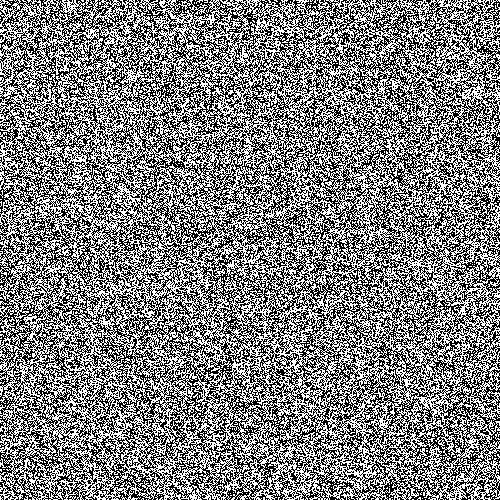
\includegraphics[width=1\textwidth]{rys.6.transfer.png}
    \caption{Przykład zmiany domeny za pomocą CycleGAN (tutaj zmiana pór roku). \protect\linebreak Żródło: \protect\url{https://junyanz.github.io/CycleGAN/}}
    \label{fig:mesh6}
\end{figure}

% ############## Uczenie się przez transfer ###############
\section{Uczenie się przez transfer}
\label{cha:cha3.5}

Ludzie mają wrodzoną zdolność wykorzystywania wiedzy, którą zdobyli w~trakcie wykonywania innego zadania. To znaczy, wiedzę, którą zdobywamy, ucząc się pewnej rzeczy, możemy wykorzystać, wykonując inne, aczkolwiek powiązane zadanie. Im bardziej powiązane są te zadania, tym łatwiej jest nam przenieść naszą wiedzę \cite{Sarkar18}. A~więc w~najprostszych słowach, uczenie się przez transfer (ang. \ita{transfer learning}) to idea wykorzystania wiedzy zdobytej w~ramach jednego zadania do rozwiązywania zadań pokrewnych. W~ostatnich latach uczenie się przez transfer również zaczęto stosować w~uczeniu maszynowym, czy też w~głębokim uczeniu \cite{Chmiel20}. W~tym przypadku najczęściej polega ono na wykorzystaniu już istniejącego modelu do nowego problemu. Jakie wynikają z~tego korzyści? Przede wszystkim to podejście pozwala nam na osiągnięcie zamierzonych rezultatów (np. wysoka skuteczność klasyfikacji) przy użyciu mniejszej ilości danych niż w~przypadku trenowania całkowicie nowego modelu. 
Uczenie się przez transfer dobrze można zilustrować na przykładzie rozpoznawania obrazów (tym lepiej, że właśnie w~tym celu wykorzystano tę metodologię w~niniejszej pracy), a~mianowicie sieci neuronowe w~początkowych warstwach wykrywają krawędzie, w~kolejnych warstwach wykrywają kształty, natomiast w~ostatnich warstwach wykrywają specyficzne zależności dla danego zadania \cite{Chmiel20}. A~więc w~celu klasyfikacji danych obiektów można skorzystać z~ogólnie znanych, dobrze wytrenowanych, na wielkich zbiorach danych, głębokich sieci neuronowych (np. \textit{VGG19}) w~ten sposób, że budujemy nowy model, który kopiuje początkowe warstwy wcześniej wytrenowanej sieci, a~następnie przyłączamy nowe warstwy, które zostaną dotrenowane w~tym konkretnym celu. Oprócz wykorzystania uczenia transferowego do klasyfikacji obrazów skutecznie stosowano to podejście również w~takich zadaniach jak klasyfikacja tekstów czy filtrowanie spamu \cite{Bickel06}. 

% ############## Wykorzystane metody uczenia maszynowego ###############
\section{Wykorzystane metody uczenia maszynowego}
\label{cha:Wykorzystane metody uczenia maszynowego}

W tym rozdziale zostaną przedstawione metody uczenia maszynowego, które zostały wykorzystane w~trakcie realizacji pracy. Większość z~nich to algorytmy uczenia nadzorowanego ze względu na charakterystykę danych.

\subsection{Maszyna wektorów nośnych}
\label{cha:Maszyna wektorów nośnych}

Maszyna wektorów nośnych (ang. \textit{support-vector machine}, SVM) to model nadzorowanego uczenia maszynowego, który wyznacza hiperpłaszczyznę w~celu rozdzielenia przykładów należących do dwóch klas z~maksymalnym marginesem \cite{Sawka20}. SVM to potężny i~wszechstronny model uczenia maszynowego, który jest w~stanie przeprowadzić klasyfikację liniową, nieliniową oraz regresję \cite{Sawka18}. Rysunek \ref{fig:mesh7} przedstawia koncepcję działania SVM. Model ten mapuje przykłady uczące do punktów w~przestrzeni tak, aby maksymalizować odległość między dwiema kategoriami. Następnie nowe przykłady są mapowane do tej samej przestrzeni i~w zależności, po której stronie marginesu się znajdują, tak są klasyfikowane. Tak jak wspomniano wyżej, za pomocą SVM również można skutecznie przeprowadzać klasyfikację nieliniową, co jest możliwe dzięki tzw. sztuczce z~funkcją jądra (ang. \textit{kernel trick}). Polega ona na tym, iż dane wejściowe są niejawnie odwzorowywane do przestrzeni cech o~wyższym wymiarze \cite{Boser92}. 

\begin{figure}[h]
    \centering
    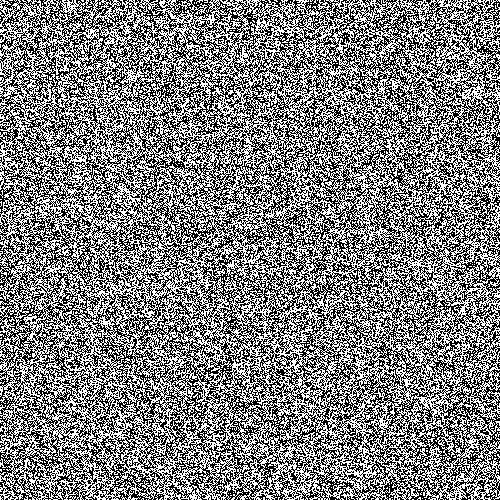
\includegraphics[width=0.5\textwidth]{rys.7.svm.png}
    \caption{Działanie SVM. H1 nie separuje klas, H2 separuje, lecz z~małym marginesem, natomiast H3 separuje z~maksymalnym marginesem \protect\linebreak 
		(źródło: \protect\href{https://en.wikipedia.org/wiki/Support-vector_machine}{https://en.wikipedia.org/wiki/Support-vector\_machine})}
    \label{fig:mesh7}
\end{figure}
\noindent Jednym z~problemów, które można napotkać w~trakcie korzystania z~SVM jest ich czułość na skalę cech. Jednakże łatwo jest to obejść przy pomocy przeskalowania cech (np. standaryzacja). Innym problemem jest konieczność posiadania całkowicie oznaczonych danych \cite{Hur02}. Dodatkowo parametry tego modelu są trudne do zinterpretowania. Mimo wszystko wady te nie są zbyt uciążliwe, a~nawet istnieją rozwiązania, które je obchodzą. Istnieje taki model, jak SVC (ang. \textit{support-vector clustering}), który można wykorzystać w~celu uczenia nienadzorowanego. Dodatkowo istnieją rozszerzenia modelu SVM, dzięki którym można wykorzystać ten model do klasyfikacji wieloklasowej. Polegają one m.in. na takich strategiach, jak rozpatrywanie danej etykiety przeciwko wszystkim pozostałym (i tak dla każdej etykiety). Algorytm SVM jest jednym z~najczęściej stosowanych w~przemyśle, dlatego jego efektywność zostanie przetestowana na tle innych algorytmów.

\subsection{Drzewo decyzyjne}
\label{cha:Drzewo decyzyjne}

Drzewo decyzyjne (ang. \textit{decision tree}, DT) to algorytm uczenia maszynowego stosowany w~celu pozyskiwania wiedzy na podstawie przykładów \cite{wiki:dec.drzewo}. Mają wiele zastosowań i~służą zarówno do zadań klasyfikacji, jak i~regresji. Jest to struktura, która kształtem przypomina drzewo (stąd nazwa), a~każda ścieżka w~tym drzewie przedstawia możliwą \textbf{ścieżkę decyzyjną} wraz z~jej skutkami \cite{Grus18}. Składa się ono z~\textbf{węzłów} (które jednocześnie oznaczają jakąś decyzję, stan) i~\textbf{gałęzi} (wybór, możliwość). Drzewo konstruowane jest od korzenia i~z każdą kolejną decyzją do podjęcia jest budowany w~dół, do tzw. \textbf{liści} (ang. \textit{leaf}), które oznaczają etykietę klasy. Istnieje wiele algorytmów generowania drzew decyzyjnych. Najbardziej znane z~nich, to \textit{ID3} (\textit{Iterative Dichotomiser 3}), czy też \textit{C4.5}. Algorytm \textit{ID3} polega na tym, że w~każdej iteracji jest wybierany niewykorzystany atrybut, który daje największy wzrost informacji (bądź np. najmniejszą miarę zanieczyszczenia), a~zbiór danych jest dzielony według wartości tego atrybutu. Natomiast algorytm \textit{C4.5} jest rozszerzeniem wcześniejszego algorytmu i~wprowadza takie usprawnienia, jak \cite{Quinlan96}:
\begin{itemize}
	\item obsługa atrybutów ciągłych i~dyskretnych,
	\item obsługa danych z~brakującymi wartościami atrybutów,
	\item przycinanie drzew po ich utworzeniu.
\end{itemize}
Wśród największych zalet drzew decyzyjnych wymienia się \cite{wiki:dec.tree}:
\begin{itemize}
	\item prosty algorytm,
	\item łatwo interpretowalne wyniki,
	\item działają nawet dla niewielkiej liczby danych,
	\item nie wymagają przygotowywania danych (w szczególności skalowania) \cite{Sawka18}.
\end{itemize}
Natomiast posiadają też wady, takie jak \cite{wiki:dec.tree}:
\begin{itemize}
	\item niestabilność (niewielka zmiana danych może prowadzić do dużej zmiany struktury drzewa),
	\item często są stosunkowo niedokładne (inne klasyfikatory zazwyczaj radzą sobie lepiej),
	\item może wystąpić problem nadmiernego dopasowania się do danych.
\end{itemize}
Pomimo tych wad klasyfikator ten zostanie wykorzystany w~badaniach, głównie ze względu właśnie na jego bardzo łatwą interpretowalność.
Jako ciekawostkę można dodać, że drzewa decyzyjne składają się na algorytm lasu losowego (ang. \textit{random forest}), który zostanie omówiony w~podrozdziale \ref{cha:Las losowy}. 

% ################ LAS LOSOWY ################
\subsection{Las losowy}
\label{cha:Las losowy}

Jak zostało wspomniane wyżej, drzewa decyzyjne mogą zbyt mocno dopasować się do danych treningowych. Jednym z~rozwiązań jest technika \textbf{lasów losowych} (ang. \textit{random forest}, RFC), która polega na tworzeniu wielu drzew decyzyjnych, a~następnie klasyfikacji w~drodze głosowania \cite{Grus18}, a~więc jako odpowiedź jest generowana dominanta klas (klasyfikacja) lub średnia przewidywana wartość (regresja) \cite{Ho95}. Istnieje kilka różnych algorytmów tworzenia lasów losowych. Jednym z~nich jest \textbf{agregacja} (ang. \textit{bagging}, \textit{bootstrap aggregating}). Polega on na tym, iż wielokrotnie wybiera się losowe podzbiory zestawu uczącego ze zwracaniem (ang. \textit{sampling with replacement}) w~celu dopasowania do każdego takiego zbioru nowego drzewa \cite{Sawka18}. Dzięki temu podejściu zmniejsza się wariancja modelu bez zwiększania obciążenia \cite{Ramchandani18}, gdyż pojedyncze drzewa decyzyjne nie są ze sobą skorelowane (dzięki uczeniu ich na różnych zbiorach danych). Następnie, w~celu klasyfikacji, wszystkie pojedyncze drzewa zwracają wynik, który jest uśredniony. Dodatkowo, aby jeszcze mocniej zmniejszyć korelację między drzewami, w~przypadku lasów losowych korzysta się ze zmodyfikowanego algorytmu trenowania drzewa, gdzie przy każdym kolejnym węźle jest wybierany losowy podzbiór cech. Dzięki temu, jeśli w~danych występuje cecha, która jest silnym predyktorem dla zmiennej przewidywanej, jej wykorzystanie w~różnych drzewach zostanie ograniczone, tym samym dalej zmniejszając korelację między nimi.

Innym podejściem jest \textbf{wzmacnianie} (ang. \textit{boosting}) \cite{aporras}. Główną różnicą między agregacją a~wzmacnianiem jest to, iż w~przypadku tego pierwszego każde drzewo jest uczone niezależnie od pozostałych i~ten etap może być przeprowadzony równolegle. Natomiast w~przypadku drugiego algorytmu uczenie pojedynczych drzew następuje sekwencyjnie i~każdy kolejny klasyfikator bierze pod uwagę wyniki poprzedniego klasyfikatora. Danym błędnie sklasyfikowanym przypisuje się większą wagę, tym samym kolejne modele zwracają większą uwagę trudnym danym. Jednakże w~przypadku wzmacniania klasyfikacja odbywa się nieco inaczej, gdyż tutaj również mamy wagi, które są przypisywane klasyfikatorom w~trakcie uczenia – im lepszy klasyfikator, tym większe wagi otrzymuje. Dzięki zastosowaniu jednego z~tych dwóch podejść zwiększa się stabilność modelu. Jednakże jeżeli mamy do czynienia z~danymi, dla których pojedyncze drzewo osiąga słabe wyniki, wtedy rozwiązaniem może być zastosowanie wzmacniania. Jeżeli zaś problemem jest nadmierne dopasowanie się drzewa do danych, wtedy pomocne może się okazać zastosowanie agregacji.

% ############### KNN #######################

\subsection{K najbliższych sąsiadów}
\label{cha:K najbliższych sąsiadów}

Algorytm $k$ najbliższych sąsiadów (ang. \textit{k-nearest neighbors algorithm}, k-NN) jest jednym z~najprostszych modeli predyktywnych \cite{Grus18}. Można go użyć zarówno do klasyfikacji, jak i~regresji. Jedynym wymaganiem tej metody jest wybór jakiejś miary odległości, a~więc jest metodą nieparametryczną. Jego działanie opiera się na założeniu, że im bliżej siebie znajdują się punkty, tym są bardziej do siebie podobne. Tak więc, dla przykładowej obserwacji liczona jest odległość (według z~góry ustalonej metryki) od pozostałych punktów i~wybieranych jest $k$ najbliższych (ustalona z~góry liczba). Następnie wybór najczęściej występującej (bądź uśrednienie wartości zmiennej objaśnianej) jako wynik klasyfikacji. Najczęściej stosuje się metrykę euklidesową, bądź też metrykę Mahalanobisa \cite{Jaskowiak70}. Jeżeli cechy danych znacznie różnią się w~skali, bądź reprezentują inne jednostki, wtedy normalizacja może znacząco poprawić dokładność \cite{Piryonesi20}. Innym ciekawym usprawnieniem może być przypisanie wag sąsiadom w~taki sposób, aby najbliżsi sąsiedzi mieli największy wpływ na wynik klasyfikacji (często stosowana jest odwrotność odległości) \cite{wiki:knn}. k-NN odnotowuje dobre wyniki w~zakresie spójności, jest łatwy w~implementacji, natomiast może być wymagający obliczeniowo w~przypadku dużych zbiorów danych \cite{wiki:knn}. Jego użyteczność jest największa w~przypadku, gdy zależność między zmiennymi objaśniającymi a~objaśnianymi jest złożona \cite{wiki:knn}. Na poniższym rysunku zostało przedstawione schematycznie działanie k-NN (rys. \ref{fig:mesh8}). Wzmacnianie zostało szegółowo omówione w~rozdziale \ref{cha:Wzmacnianie}.



\begin{figure}[h]
    \centering
    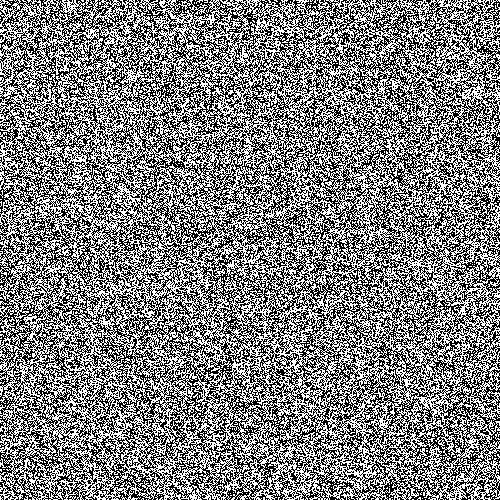
\includegraphics[width=0.5\textwidth]{rys.8.knn.png}
    \caption{Schemat działania algorytmu k-NN. Szary punkt, w~zależności od wartości $k$ i~odległości od najbliższych punktów, będzie miał przypisaną jedną z~trzech dostępnych klas (źródło \protect\href{https://medium.com/capital-one-tech/k-nearest-neighbors-knn-algorithm-for-machine-learning-e883219c8f26}{medium.com}, Madison Scott)}
    \label{fig:mesh8}
\end{figure}

% ############## LOGIT ###################

\subsection{Regresja logistyczna}
\label{Regresja logistyczna}

Regresja logistyczna (ang. \textit{logistic regression}) to model używany w~statystyce do przewidywania prawdopodobieństwa pewnej klasy bądź zdarzenia, które może przyjmować tylko dwie wartości \cite{wiki:logit}. Mechanizm działania tej metody jest podobny do regresji liniowej, tyle że tutaj wyliczamy ważoną sumę cech wejściowych (wzór \ref{eq.logit})

\begin{equation}
\label{eq.logit}
logit(p_{i}) = ln( \frac {p_{i}} {1-p_{i}}) = \beta_{1}x_{1, i}+\dots+\beta_{k}x_{k, i}
\end{equation}

\noindent gdzie $p_i$ to nieznane prawdopodobieństwo sukcesu w~próbie $i$, $x_{k,i}$ to wartość $k$-tego predyktora próby $i$, natomiast $\beta_k$ to nieznany parametr $k$-tego predyktora, który jest optymalizowany (najczęściej za pomocą metody największej wiarygodności) \cite{Menard02}. Następnie zwracana jest wartość funkcji logistycznej z~tego rezultatu (wzór \ref{eq.sigma}) \cite{Sawka18}, co jest równoznaczne z~oszacowaniem prawdopodobieństwa: 

\begin{equation}
\label{eq.sigma}
	\hat p = \sigma(t)=\frac {1} {1+exp(-t)}
\end{equation}

\noindent Następnie prognoza modelu regresji logistycznej jest wyliczana za pomocą wzoru \ref{eq.logit.prognoza}.

\begin{equation}
\label{eq.logit.prognoza}
\hat {y} =
	\begin{cases}
	      0 & \text{jeśli $\hat {p} < 0.5$}\\
	      1 & \text{wpp.}
	\end{cases}       
\end{equation}

\noindent Model ten może zostać rozszerzony tak, aby przewidywał kilka klas zdarzeń w~taki sposób, iż każdemu zdarzeniu jest przypisywane prawdopodobieństwo, a~suma wszystkich tych prawdopodobieństw wynosi jeden. W~tym celu wykorzystuje się funkcję \textit{softmax} (wzór \ref{eq.softmax}), przekazując jej prawdopodobieństwa wystąpienia każdej klasy (nie muszą się sumować do jedynki), następnie dla każdej jest liczona eksponenta, po czym następuje normalizacja (dzieląc wyniki przez sumę wszystkich eksponent) \cite{Sawka18}:

\begin{equation}
\label{eq.softmax}
\sigma(z)_i=\frac {e^{z_i}} { 
    \sum \limits_{j=1}^{K} e^{z_j}}
\end{equation}

\noindent gdzie $z$ to wektor zawierający wyniki każdej klasy, $i$ to ustalona klasa. Jak wspomniano wcześniej, współczynniki są estymowane za pomocą metody największej wiarygodności, gdzie w~sposób iteracyjny (np. metoda Newtona) modyfikowane są wartości współczynników \cite{Menard02}. Ostatnim elementem jest uczenie modelu. Jego celem jest uzyskanie modelu, który zwraca wysokie prawdopodobieństwo dla klasy docelowej. W~tym celu minimalizuje się funkcję kosztu zwaną entropią krzyżową (ang. \textit{cross entropy}), przedstawioną poniżej (wzór \ref{eq.xentropy}):

\begin{equation}
\label{eq.xentropy}
	H=-\sum \limits_{c=1}^{M}y_{o,c}log(p_{o,c})
\end{equation}

\noindent gdzie $M$ oznacza liczbę klas, $y$ to wskaźnik binarny ($0$ lub $1$ w~zależności czy etykieta $c$ jest zgodna z~klasą obserwacji $o$) oraz $p$ to przewidywane prawdopodobieństwo przypisania klasy $c$ obserwacji $o$.

Regresja logistyczna jest bardzo skuteczna dla prostych zbiorów danych, a~także w~przypadku zbiorów liniowo separowalnych. Dodatkowo jej współczynniki mogą być interpretowane jako wskaźniki ważności cech, dlatego również zostanie uwzględniona w~badaniach.


% ############ BAYES ###############

\subsection{Naiwny klasyfikator bayesowski}
\label{cha:Naiwny klasyfikator bayesowski}

Naiwny klasyfikator bayesowski (ang. \textit{naive Bayes classifier}) należy do rodziny prostych probabilistycznych klasyfikatorów, które opierają się na twierdzeniu Bayesa \cite{wiki:bayes}. Istotnym założeniem tego modelu jest wzajemna niezależność predyktorów. Naiwne klasyfikatory bayesowskie są wysoce skalowalne, aczkolwiek wymagają wielu parametrów liniowych w~stosunku do liczby zmiennych) \cite{wiki:bayes}. Dużym atutem tego modelu jest zastosowanie metody największej wiarygodności, przez co czas uczenia jest liniowy (w przeciwieństwie do wielu innych typów klasyfikatorów) \cite{wiki:bayes}, dodatkowo nie trzeba akceptować prawdopodobieństwa bayesowskiego. Kolejną przewagą nad innymi modelami jest niska wymagana liczba danych uczących, aby model mógł wyestymować parametry potrzebne do klasyfikacji \cite{wiki:bayes}. Korzystając z~twierdzenia Bayesa można wyprowadzić wzór, który stoi za naiwnym modelem probabilistycznym Bayesa (wzór \ref{eq.bayes}):

\begin{equation}
\label{eq.bayes}
	p(C|F_1,\dots,F_n)=\frac 1 Zp(C)\prod_{i=1}^{n}p(F_i|C)
\end{equation}

\noindent gdzie $C$ to dana klasa zmiennej zależnej, $n$ to liczba zmiennych niezależnych, $F1,\dots,F_n$ to zmienne niezależne, natomiast $Z$ jest współczynnikiem skalowania zależnym od predyktorów \cite{wiki:bayes}. Klasyfikacja odbywa według poniższej funkcji (wzór \ref{eq.bayes.clf}):

\begin{equation}
\label{eq.bayes.clf}
	\hat y=\underset{k}{\arg\max}\ p(C_k)\prod_{i=1}^{n}p(x_i|C_k)
\end{equation}

\noindent gdzie $\hat{y}$ to przewidywana klasa, $n$ to liczba zmiennych niezależnych. Pomimo faktu, że wymogi niezależności są często łamane, naiwny klasyfikator bayesowski posiada szereg cech, które w~rzeczywistości są zaskakująco korzystne. Klasyfikacja jest poprawna, podobnie jak w~przypadku wszystkich klasyfikatorów probabilistycznych, które wykorzystują metodę maksimum prawdopodobieństwa \textit{a posteriori} (MAP), o~ile właściwa klasa jest bardziej prawdopodobna niż pozostałe. A~więc klasyfikator jest wystarczająco silny, aby zignorować główne wady naiwnego modelu probabilistycznego \cite{wiki:bayes}.

% ################# WZMACNIANIE ###################

\subsection{Wzmacnianie}
\label{cha:Wzmacnianie}

Wzmacnianie (ang. \textit{boosting}) zostało już pokrótce omówione przy okazji lasów losowych (rozdział \ref{cha:Las losowy}). W skrócie, polega ono na pracy zespołowej wielu słabych klasyfikatorów, otrzymując w~ten sposób zespół będący silnym klasyfikatorem. Istotą wzmacniania jest sekwencyjne uczenie predyktorów w~taki sposób, że każdy kolejny próbuje poprawiać błędy poprzednika \cite{Sawka18}. W~poniższych podrozdziałach zostaną przedstawione dwa najpopularniejsze algorytmy wzmacniania: \textit{AdaBoost} oraz wzmacnianie gradientowe (ang. \textit{gradient boosting}). 

% ################ AdaBoost ####################

\subsubsection{AdaBoost}
\label{AdaBoost}

Ideą tego modelu jest uczenie sekwencyjne kolejnych klasyfikatorów w~taki sposób, że każdy kolejny próbuje korygować błędy swojego poprzednika. To znaczy, każdy kolejny klasyfikator przykłada większą wagę przykładom uczącym, dla których poprzedni algorytm został niedotrenowany \cite{Sawka18}. W~ten sposób do zespołu są dołączane coraz bardziej dokładne klasyfikatory, tym samym zwiększając jego skuteczność. Ostatecznie prognoza jest średnią ważoną wyników poszczególnych klasyfikatorów. Ogólny schemat jest przedstawiony poniżej.

Początkowo każdej próbce jest przypisywana waga (wzór \ref{eq.waga.adaboost}):

\begin{equation}
\label{eq.waga.adaboost}
	w^{(i)}=\frac 1 m
\end{equation}

\noindent gdzie $m$ to liczba próbek. Należy również pamiętać, że suma wszystkich wag wynosi zawsze jeden. Po wytrenowaniu pierwszego klasyfikatora zostanie mu przypisany ważony współczynnik błędu $r_j$, gdzie $j$ oznacza liczbę porządkową klasyfikatora (równanie \ref{eq.wsp.bledu}):

\begin{equation}
\label{eq.wsp.bledu}
	r_j = \frac { \sum\limits_{\substack{i=1 \\ \hat y_j^{(i)} \neq y^{(i)}}}^{m} w^{(i)}}{{\sum\limits_{i=1}^{m} w^{(i)}}}
\end{equation}

\noindent gdzie $\hat y_j^{(i)}$ jest prognozą $j$-tego klasyfikatora dla $i$-tego przykładu. Następnie zgodnie z~równaniem \ref{eq.wagi.clf.adaboost} wyliczana jest waga dla $j$-tego klasyfikatora:

\begin{equation}
\label{eq.wagi.clf.adaboost}
	\alpha_j=\eta log\frac {1-r_j} {r_j}
\end{equation}
gdzie $\eta$ to współczynnik uczenia. W~ten sposób dokładniejsze klasyfikatory dostają 
większe wagi, natomiast te mniej dokładne – mniejsze. Wykres tego równania został przedstawiony na rysunku \ref{fig:mesh9}.
\begin{figure}[h]
    \centering
    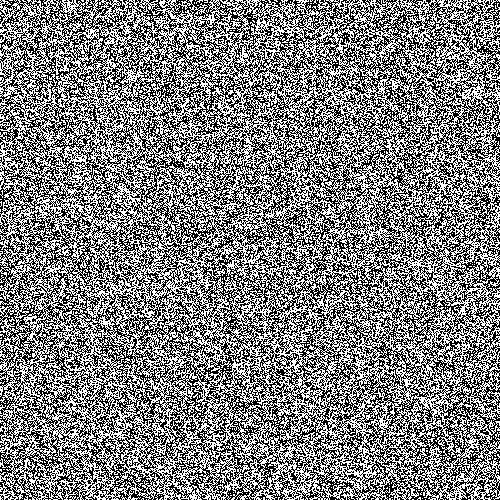
\includegraphics[width=0.6\textwidth]{rys.9.png}
    \caption{Wykres równania \ref{eq.wagi.clf.adaboost}. Widać, że dla błędów zerowych waga klasyfikatora zbiega się do nieskończoności, natomiast dla błędów dążących do jedynki, waga zbiega się do minus nieskończoności (źródło: opracowanie własne)}
    \label{fig:mesh9}
\end{figure}
W~kolejnym etapie następuje aktualizacja wag próbek (równanie \ref{eq.adaboost.aktualizacja.wag}):
\begin{equation}
	\label{eq.adaboost.aktualizacja.wag}
	w^{(i+1)} =
	\begin{cases}
		w^{(i)} & \text{gdy } \hat {y}_j^{(i)} = y^{(i)}\\
		w^{(i)}exp(\alpha_j) & \text{wpp.}
	\end{cases}
\end{equation}
Cały ten proces jest powtarzany wielokrotnie, iteracyjnie, aż osiągniemy ustaloną liczbę klasyfikatorów bądź też wyniki zwracane przez model będą na odpowiednim
poziomie (zazwyczaj uczenie zatrzymuje się przy $100\%$) \cite{Sawka18}. Ostatecznie, w~celu klasyfikacji jest liczona średnia ważona (przy użyciu wag z~równania \ref{eq.wagi.clf.adaboost}) z~predykcji wszystkich klasyfikatorów składających się na model i~wybierana jest odpowiedź, która otrzyma tym sposobem najwięcej głosów (równanie \ref{eq.adaboost.klasyfikacja}):

\begin{equation}
\label{eq.adaboost.klasyfikacja}
\hat y (x) = \underset{k}{\arg\max} \sum_{\substack{j=1 \\ \hat y_j(x)=k}}^N \alpha_j
\end{equation}

\noindent gdzie $N$ to liczba klasyfikatorów. 

Podsumowując, AdaBoost ma wiele zalet. Wśród nich znajduje się ta, iż AdaBoost nie wymaga modyfikowania parametrów w~celu osiągnięcia optymalnego modelu (w przeciwieństwie do np. SVM). Dodatkowo, AdaBoost może być stosowany, gdy chcemy poprawić dokładność słabego klasyfikatora \cite{Kurama20}. Jednak trzeba pamiętać o~tym, iż metody wzmacniania działają progresywnie, a~więc wymagane są dane wysokiej jakości. Dodatkowo należy się wcześniej upewnić, że usunięto wszystkie wartości odstające (ang. \textit{outliers}), na które ten model również jest wrażliwy \cite{Kurama20}. 

% ################## WZMACNIANIE GRADIENTOWE ##################

\subsubsection{Wzmacnianie gradientowe}
\label{cha:Wzmacnianie gradientowe}

Wzmacnianie gradientowe (ang. \textit{gradient boosting}) to inna bardzo popularna technika wzmacniania \cite{Sawka18}. Nadaje się zarówno do klasyfikacji, jak i~regresji. Podobnie do poprzedniej metody, polega na dodawaniu kolejnych klasyfikatorów do zespołu w~sposób sekwencyjny w~taki sposób, że następnik poprawia poprzednika. Różnicą między tą techniką a~AdaBoost jest to, że tutaj nie aktualizujemy wag przykładów po każdym przebiegu, lecz próbujemy dopasować predyktor do błędu resztowego (ang. \textit{residual error}) popełnionego przez poprzedni klasyfikator \cite{Sawka18}. Zwyczajowo jako słabych predyktorów używa się drzew decyzyjnych, a~otrzymany algorytm jest nazywany gradientowo wzmocnionym drzewem (ang. \textit{gradient boosted tree}). Wyniki uzyskiwane za pomocą tej techniki zazwyczaj są lepsze od tych uzyskiwanych za pomocą lasów losowych \cite{Piryonesi19}. Jedno z~prostszych wyjaśnień tej metody przedstawił Cheng Li na przykładzie regresji \cite{Li}. Załóżmy, że chcemy nauczyć model $F$ przewidywać wartości postaci (\ref{eq.gradient.model}):
\begin{equation}
	\label{eq.gradient.model}
	\hat y = F(x)
\end{equation}
minimalizując błąd średniokwadratowy (\ref{eq.gradient.mse}):
\begin{equation}
	\label{eq.gradient.mse}
	L=\frac 1 n \sum_{i=1}^n(\hat y_i-y_i)^2
\end{equation}
gdzie:
\begin{eqwhere}[2cm]
	\item $n$ to liczba próbek w~zbiorze uczącym $y$,
	\item $\hat y_i$ to wartość przewidywana $F(x)$,
	\item $\hat y_i$ to obserwowana wartość.
\end{eqwhere}
Zakładając, iż algorytm składa się z~$M$ etapów, w~każdym etapie $m$ ($1<m<M$) wzmacniania istnieje niedoskonały model $F_m$. W~celu poprawienia jakości modelu $ F_m$ dodaje się pewien estymator $h_m(x)$ (równanie \ref{eq.gradient.estimator}):
\begin{equation}
	\label{eq.gradient.estimator}
	h_m(x)=y-F_m(x)
\end{equation}
W ten sposób $h$ dopasowuje się reszty $y-F_m(x)$ (zwanej błędem resztowym) przyczyniając się do polepszania wyników osiąganych przez kolejne modele. Rozszerzenie tej idei do klasyfikacji polega na obserwacji, iż reszty $h_m(x)$ to tak naprawdę ujemny gradient błędu średniokwadratowego (równania \ref{eq.gradient.mse2}, \ref{eq.gradient.mse.partial}):
\begin{equation}
\label{eq.gradient.mse2}
L_{MSE}=\frac 1 2(y-F(x))^2
\end{equation}
\begin{equation}
\label{eq.gradient.mse.partial}
h_m(x)=-\frac {\partial L_{MSE}} {\partial F}=y-F(x)
\end{equation}
Wzmacnianie gradientowe to szeroko wykorzystywany algorytm. Jednak trzeba pamiętać, iż mimo że zazwyczaj podnosi dokładność modelu, to jednak tracimy na interpretowalności, dodatkowo rośnie czas uczenia.

% ########### SIECI NEURONOWE ##############

\subsection{Sieci neuronowe}
\label{cha:Siecineuronowe}

Sztuczne sieci neuronowe (ang. \textit{artificial neural networks}), zwykle nazywane po prostu \textbf{sieciami neuronowymi} (ang. \textit{neural networks}), to systemy komputerowe inspirowane biologicznymi sieciami neuronowymi, na które się składają mózgi zwierząt \cite{Tadeusiewicz15}. Główną zaletą tych systemów jest ich możliwość rozwiązywania problemów, nie będąc bezpośrednio do tego zaprogramowanymi. Najprostszym elementem sieci neuronowych jest sztuczny neuron. Każdy neuron posiada wiele wejść i~pojedyncze wyjście, które może być przesyłane do wielu pozostałych neuronów. Wejściem mogą być jakieś cechy (np. wiek, wzrost), natomiast wyjściem ostatnich neuronów, które realizują jakieś zadanie, może być np. wynik klasyfikacji (np. płeć). Aby obliczyć wyjście neuronu, każde jego wejście jest przemnożone przez \textbf{wagę} połączenia z~poprzednim neuronem, następnie dodawana jest wartość zwana \textbf{obciążeniem} (ang. \textit{bias}), a~na końcu ta wartość jest przekazywana do tzw. \textbf{funkcji aktywacji} (ang. \textit{activation function}), której wynik jest jednocześnie wyjściem neuronu. Schemat neuronu został przedstawiony na rys~\ref{fig:mesh10}.
\begin{figure}[h]
    \centering
    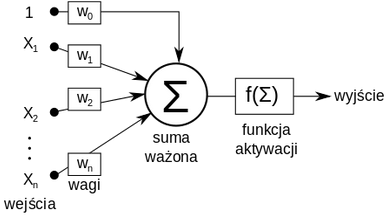
\includegraphics[width=0.6\textwidth]{rys.10.neuron.png}
    \caption{Schemat neuronu McCullocha-Pittsa (źródło: \protect\href{https://pl.wikipedia.org/wiki/Neuron_McCullocha-Pittsa}{wikipedia}, Krzysztof Zajączkowski)}
    \label{fig:mesh10}
\end{figure}
Kolejnym elementem są \textbf{połączenia} (ang. \textit{connections}) oraz \textbf{wagi} (ang. \textit{weights}). Sieć składa się z~połączeń, które łączą neurony z~poszczególnych warstw, dostarczając wyjście neuronów z~warstwy poprzedniej. Jak wcześniej zostało napisane, neuron może mieć tylko jedno wyjście, tzn. jedną wartość wyjścia, natomiast może przekazywać tę wartość wielu neuronom w~kolejnej warstwie. Za pomocą wag i~połączeń są przekazywane wartości z~warstw poprzedzających do warstw następnych. Wykorzystuje się tutaj mechanizm zwany \textbf{funkcją propagacji} (ang. \textit{propagation function}). Jak wspomniano wcześniej, neurony znajdują się w~\textbf{warstwach} (ang. \textit{layers}). Neurony z~danej warstwy łączą się tylko z~neuronami z~warstwy poprzedniej oraz neuronami z~warstwy następnej (w standardowych implementacjach). Warstwa, która na wejściu otrzymuje dane jest nazywana \textbf{warstwą wejściową} (ang. \textit{input layer}), natomiast warstwa, która zwraca wyniki jest nazywana warstwą wyjściową (ang. \textit{output layer}). Pomiędzy tymi warstwami może być zero lub więcej warstw, które są nazywane \textbf{warstwami ukrytymi} (ang. \textit{hidden layers}). Schemat sieci neuronowej został przedstawiony na poniższym obrazku (rys. \ref{fig:mesh11}). 
\begin{figure}[h]
    \centering
    \includegraphics[width=0.9\textwidth]{rys.11.sieć.png}
    \caption{Schemat sieci neuronowej (źródło: \protect\url{https://www.controlengineering.pl}, Jimmy W. Key)}
    \label{fig:mesh11}
\end{figure}
Uczenie takich sieci polega na modyfikacji wag połączeń w~taki sposób, aby sieć coraz lepiej dopasowywała się do danych uczących. Wagi modyfikowane są tak, aby zmniejszać błąd zwracany przez tak zwaną \textbf{funkcję straty} (ang. \textit{loss function}), która zwraca błąd sieci dla każdej pojedynczej instancji wejściowej (bądź partii wejściowej). Odbywa się to za pomocą \textbf{propagacji wstecznej} (ang. \textit{backpropagation}). Polega ona na obliczeniu gradientu z~\textbf{funkcji kosztu} (ang. \textit{cost function}), czyli z średniej funkcji straty dla wielu próbek, dla danych próbek wejściowych względem wag. 

Każdą sieć definiuje zestaw \textbf{hiperparametrów} (ang. \textit{hyperparameters}). Są to stałe wartości ustalane przed procesem uczenia. Odpowiednio manipulując wartościami hiperparametrów możemy uzyskać lepsze modele. Najważniejszymi hiperparametrami są:
\begin{itemize}
\item
szybkość uczenia się (ang. \textit{learning rate}) – gdy sieć popełnia błąd, modyfikowane są wagi połączeń w~taki sposób, aby zbliżyć się do poprawnego wyniku. Ten hiperparametr określa jak duży krok powinna wykonać sieć w~kierunku minimalizacji błędu,

\item
liczba ukrytych warstw (ang. \textit{hidden layers}) – za pomocą tego hiperparametru możemy zdecydować jaka powinna być architektura sieci (głębsza, dla wielkich i~skomplikowanych danych bądź płytsza, dla prostych danych),

\item
wielkość partii (ang. \textit{batch size}) – określa liczbę próbek, które są propagowane przez sieć. Ma to wpływ na wykorzystywaną pamięć, prędkość uczenia się, a~także na finalną dokładność. 
\end{itemize}
\noindent Tak jak w~przypadku klasycznych metod uczenia maszynowego, tak samo w~przypadku sieci neuronowych można skorzystać z~różnych typów uczenia (patrz rozdział \ref{cha:cha3.2}). 

\subsubsection{VGG19}
\label{cha:VGG19}

W badaniach wykorzystano sieci neuronowe, jednakże mała liczba posiadanych danych spowodowała, że konieczne było użycie techniki zwanej uczeniem się przez transfer (rozdział \ref{cha:cha3.5}). W~tym celu wykorzystano znaną architekturę, a~mianowicie VGG19 (ang. \textit{Visual Geometry Group}, 19 to liczba trenowalnych warstw) \cite{Simonyan15}. Dodatkowo na końcu architektury dodano kilka warstw, za pomocą których można wykonać \textbf{strojenie} (ang. \textit{fine tuning}), a~więc dopasowanie modelu do własnych danych. Sieć ta była trenowana w~celu klasyfikacji zdjęć w~turnieju \textit{ImageNet Large Scale Visual Recognition Challenge} (ILSVRC) w~roku 2014. Na wejściu przyjmowała obrazki w~formacie RGB (ang. \textit{red, green, blue}) o~rozmiarze $224~x~224$ (rys. \ref{fig:mesh12}). 
\begin{figure}[h]
    \centering
    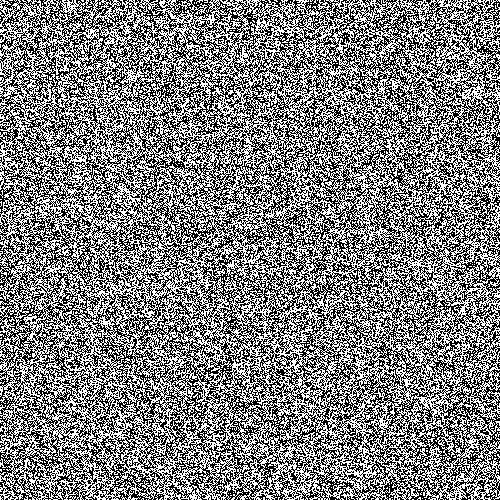
\includegraphics[width=0.8\textwidth]{rys.12.vgg.arch.png}
    \caption{Konfiguracje sieci VGG (w kolumnach). Głębokość architektury rośnie od lewej do prawej. Warstwy konwolucyjne zostały oznaczone jako „conv<rozmiar pola odbiorczego>-<liczba kanałów>”. Została również zastosowana funkcja aktywacji ReLU. Żródło: \cite{Simonyan15}}
    \label{fig:mesh12}
\end{figure}
Model ten dobrze uogólnia się dla innych zadań i zbiorów danych \cite{Simonyan15}, i~chociaż minęło już kilka lat od momentu jego wydania, wciąż osiąga wysokie wyniki w~zadaniach klasyfikacji obrazów, dlatego jego skuteczność zostanie przetestowana na tle klasycznych algorytmów uczenia maszynowego. 

\subsection{Pozostałe zagadnienia}
\label{Pozostałe zagadnienia}

W tej sekcji zostaną omówione różne techniki oraz metody wykorzystane w~trakcie badań. Zostaną też wytłumaczone niektóre pojęcia, które obejmują swoim zakresem wiele tematyk i~niepraktyczne byłoby tworzenie dla każdego problemu osobnego rozdziału.

%\subsubsection{Metryki}
%\label{metryki}
% [bla bla] można by napisac mysle 


\subsubsection{Optymalizacja hiperparametrów}
\label{Optymalizacja hiperparametrów}

Hiperparametry zostały zgrubnie omówione w~rozdz. \ref{cha:Siecineuronowe}. Przypomnijmy, że są to parametry, które kontrolują proces uczenia się i~są ustalane przed uczeniem. W~zależności od ich konfiguracji wyniki mogą się znacznie różnić. Stąd takie ważne jest, aby odpowiednio dobrać ich wartości. W~jaki sposób się to robi? Osoby dowiadczone mogą od razu ustawić odpowiednie wartości dzięki swojej praktyce. Natomiast aby mieć pewność, można skorzystać z~dostępnych metod. Istnieje ich wiele, natomiast tutaj zostanie przedstawiona jedna, która została wykorzystana w~niniejszej pracy: mowa o~przeszukiwaniu siatki (ang. \ita{grid search}). Metoda ta polega na gruntownym przeszukiwaniu (ang. \ita{exhaustive searching}) ręcznie przygotowanego podzbioru przestrzeni hiperparametrów algorytmu uczącego \cite{Hsu03}. Następnie dla każdego zestawu hiperparametrów zostaje wytrenowany model na danych uczących, po czym jego skuteczność zostaje zweryfikowana na podstawie rezultatów otrzymanych podczas ewaluacji modelu z~wykorzystaniem danych testowych.

\subsubsection{Sprawdzian krzyżowy}
\label{cross.validation}

Sprawdzian krzyżowy (ang. \ita{cross-validation}) jest to metoda statystyczna, w~której dzieli się próbę statystyczną na podzbiory, po czym przeprowadza się analizy, ale tylko na niektórych z~nich. Te, które się wykorzystuje nazywane są zbiorem uczącym, natomiast pozostałe dane służą do weryfikacji poprawności wyników i~nazywane są one danymi testowymi. Istnieje wiele rodzajów walidacji krzyżowej, aczkolwiek w~niniejszej pracy został wykorzystany jeden, a~mianowicie sprawdzian $k$-krotny. Polega ona na podziale oryginalnej próby na \ita{k} podzbiorów, po czym kolejno każdy z~nich występuje jako zbiór testowy, podczas gdy pozostałe razem jako zbiór uczący. Następnie wykonuje się analizę (\ita{k} razy), a~uzyskane \ita{k} rezultaty łączy się, np. uśredniając wyniki, dzięki czemu są one bardziej wiarygodne, a~także otrzymujemy jeden wynik.

%\subsubsection{}
%\label{}


%\subsubsection{}
%\label{}


%\subsubsection{}
%\label{}
